\section{Design of the Wah-Wah Effect}

\subsection{Choice of the Bandpass Filter}

The block diagram of the wah-wah effect has been presented in the analysis and is shown again below in  \autoref{fig:wah_diag_2}:

\begin{figure} [htbp]
	\centering
	\begin{picture}(0,0)%
	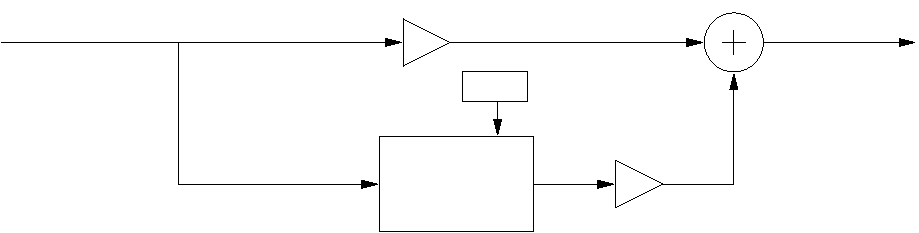
\includegraphics{wah_diag.pdf}%
	\end{picture}%
	\setlength{\unitlength}{4144sp}%
	%
	\begingroup\makeatletter\ifx\SetFigFont\undefined%
	\gdef\SetFigFont#1#2#3#4#5{%
		\reset@font\fontsize{#1}{#2pt}%
		\fontfamily{#3}\fontseries{#4}\fontshape{#5}%
		\selectfont}%
	\fi\endgroup%
	\begin{picture}(6999,1770)(2689,-2233)
	\put(6841,-1591){\textit{Wah-Wah Gain}}%
	\put(5626,-2041){$Filter$}%
	\put(6136,-1186){\textit{LFO or Pedal}}%
	\put(2746,-646){$Input$}%
	\put(8686,-646){$Output$}%
	\put(5626,-1816){$Bandpass-$}%
	\put(5986,-646){$Gain$}%
	\end{picture}%
	\caption{Block diagram of the wah-wah effect}
	\label{fig:wah_diag_2}
\end{figure}

In signal processing, different types of filters can be implemented using the first and second order allpass filters. In the case of the wah-wah, it can be inferred from \autoref{fig:wah_diag_2} that a bandpass filter is need where the center frequency is controller in order to choose where the filter is working in the frequency spectrum. \\

With a first order allpass filter, it is possible to design a circuit to make  lowpass and highpass filter but not bandpass or bandreject. Thus, the focus will be on the second order allpass filter since a bandpass one is needed. 

\begin{figure} [htbp]
	\centering
	\begin{picture}(0,0)%
	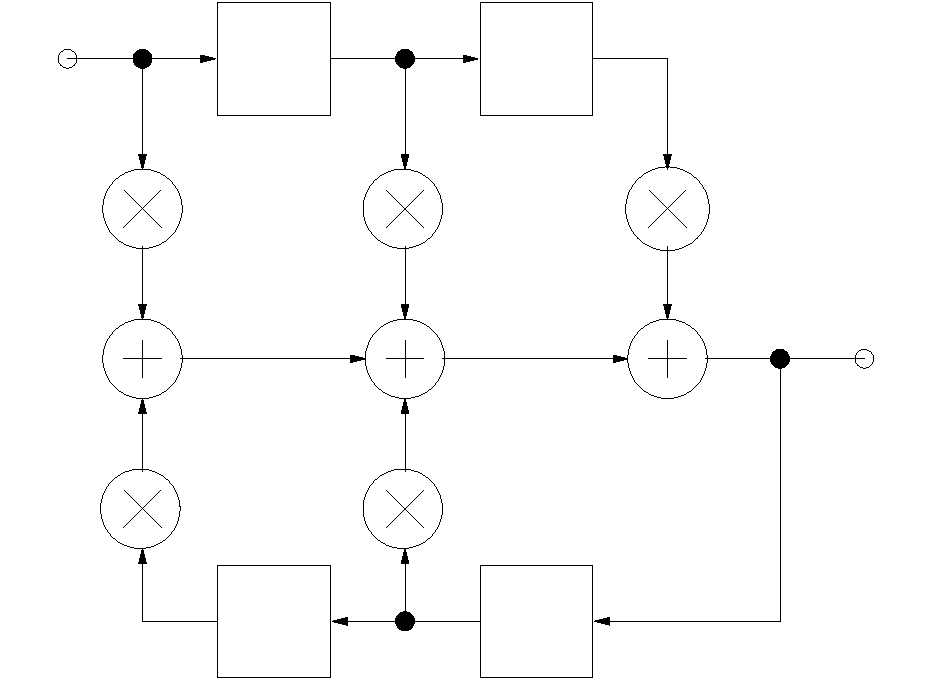
\includegraphics{wah_allpass.pdf}%
	\end{picture}%
	\setlength{\unitlength}{3947sp}%
	%
	\begingroup\makeatletter\ifx\SetFigFont\undefined%
	\gdef\SetFigFont#1#2#3#4#5{%
		\reset@font\fontsize{#1}{#2pt}%
		\fontfamily{#3}\fontseries{#4}\fontshape{#5}%
		\selectfont}%
	\fi\endgroup%
	\begin{picture}(7524,5424)(1411,-5923)
	\put(3001,-2236){-c}%

	\put(3526,-1036){T}%

	\put(5626,-1036){T}%

	\put(5626,-5536){T}%
	
	\put(3526,-5536){T}%
	
	\put(8551,-3436){y(n)}%
	
	\put(1426,-1036){x(n)}%
	
	\put(4426,-811){x(n-1)}%
	
	\put(6451,-811){x(n-2)}%
	
	\put(2251,-5686){y(n-2)}%
	
	\put(4426,-5761){y(n-1)}%
	
	\put(7201,-2236){1}%
	
	\put(3001,-4636){c}%
	
	\put(5101,-4636){-d(1-c)}%
	
	\put(5101,-2236){d(1-c)}%
	
	\end{picture}%
	\caption{Block diagram for a second-order allpass filter \citep{DAFX}}
	\label{fig:wah_allpass}
\end{figure}